\documentclass[a5paper, 20pt]{article}
\def\MakeUppercaseUnsupportedInPdfStrings{\scshape}
\usepackage[warn]{mathtext}
\usepackage{cmap}
\usepackage[T2A]{fontenc}
\usepackage[utf8]{inputenc}
\usepackage[russian]{babel}
\usepackage{amsmath}
\usepackage[ warn ]{ mathtext }
\usepackage{amsfonts}
\usepackage{amssymb}
\usepackage[normalem]{ulem}
\usepackage[pdftex]{graphics}
\usepackage{graphicx}
\usepackage{wrapfig}
\usepackage{amsmath,systeme}
\usepackage{comment}
\usepackage{slashbox}
\usepackage{pgfplots}
\usepackage{setspace}
\usepackage{geometry}
\usepackage[unicode, pdftex]{hyperref}
\usepackage{yfonts}
\usepackage{array}
\newtheorem{theorem}{Теорема}
\pgfplotsset{compat=newest}
\usepgfplotslibrary{fillbetween}
\geometry{verbose,a4paper,tmargin=2cm,bmargin=2cm,lmargin=2.5cm,rmargin=1.5cm}
\setcounter{MaxMatrixCols}{25}
\hypersetup{
    colorlinks = true,
    linkbordercolor = {white},
    linkcolor=blue
}
\usepackage[unicode, pdftex]{hyperref}
\setstretch{1.25}
\newcolumntype{P}[1]{>{\centering\arraybackslash}p{#1}}


\begin{document}
\section{Завдання 1.}

\begin{enumerate}

\item Провести аналіз вибірки та вибрати підходящу лінійну регресійну модель. 

\item За методом найменших квадратів знайти оцінки параметрів вибраної моделі.

\item На рівні значущості $\alpha = 0.05$ перевірити адекватність побудованої моделі. 

\item Для найменшого значення параметра побудованої моделі на рівні значущості $\alpha = 0.05$ перевірити гіпотезу про його значущість.

\item Побудувати прогнозований довірчий інтервал з довірчою ймовірністю $g = 0.95$ для середнього значення відклику та самого значення відклику в деякій точці, яку треба обрати самому.

\item Написати висновки.
\end{enumerate}

\begin{center}
\begin{tabular}{|c|c|c|c|c|c|c|c|} 
\hline
X & 2.15   & 2.87 & 3.55 & 5.14 & 6.25 &  7.07  &  7.83  \\ \hline
Y & 15.24 & 11.9 &  8.6  &  5.6  &  7.9  & 12.54 & 15.88 \\ \hline
\end{tabular}
\end{center}


\subsection{ Провести аналіз вибірки та вибрати підходящу лінійну регресійну модель. }

\begin{figure}[h]
\centering
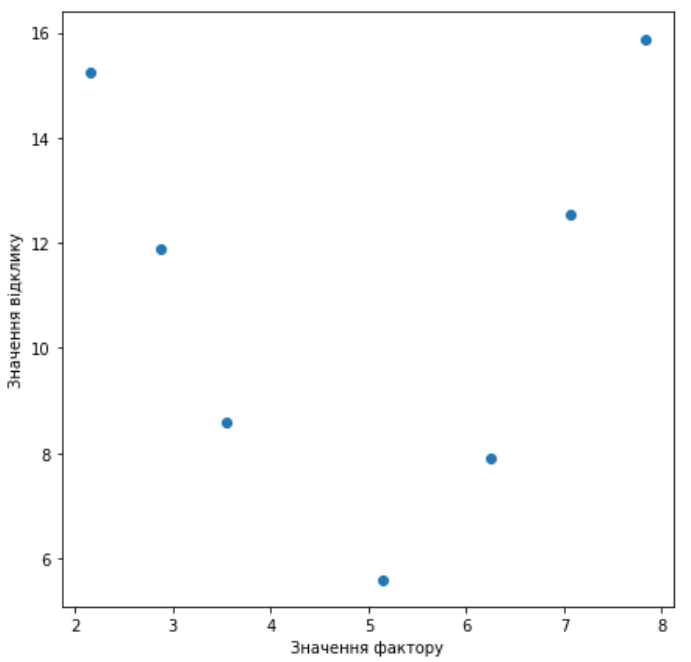
\includegraphics[scale=0.54]{plot_for_first_task_1}
\centering
\end{figure}

За розташуванням точок на діаграмі розсіювання, бачимо що точки на площині розташовані не лінійно, а більше нагадують параболу. Розглянемо модель такого вигляду:

$$f(x) = \beta_0 + \beta_1 x + \beta_2 x^2$$

Мною вибрана лійнійна регресійна модель з такими базисними функціями: $\left\{1, x, x^2\right\}$. Для підвищення "точності" моделі можна було б розглядати поліноміальну модель з більшим макимальним сетепенем. В такому випадку модель проходила би ближче до точок зображених на діаграмі розсіювання, але таке ускладнення моделі може призвести до перенавчання(англійською - overfitting). Цей термін означає, що модель на нових значеннях факторів буде погано оцінювати функцію $f(x) = \mathbb{E}(\eta/\xi = x_i)$

\newpage{}

Наглядно перенавчання продемонстровано на рисунках нище. Там червні точки це точки "значення фактору - значення відклику". Сині лінії це поліноміальні регресійні моделі з максимальним степенем - М. 

\begin{figure}[h]
\centering
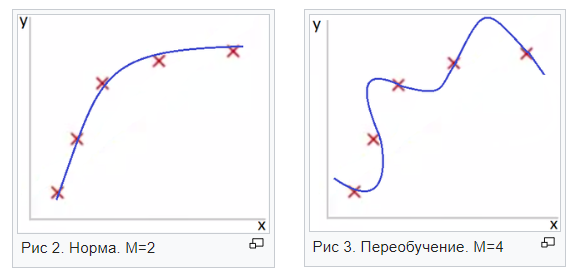
\includegraphics[scale=1]{overfitting_example}
\centering
\end{figure}

У випадку, якщо вибрана модель не пройде перевірку на адекватність, то виберемо іншу, яка має більший степінь. 

\subsection{ За методом найменших квадратів знайти оцінки параметрів вибраної моделі.}

Знайдемо матрицю плану для вибраної моделі:

$$
F =
\begin{pmatrix}
1 & 1 & 1 & 1  & 1 & 1 & 1 \\ 
2.15   & 2.87 & 3.55 & 5.14 & 6.25 &  7.07  &  7.83 \\
2.15^2   & 2.87^2 & 3.55^2 & 5.14^2 & 6.25^2 &  7.07^2  &  7.83^2
\end{pmatrix}^T
$$

Оскільки $rang  F = 3$, то для того, щоб ми могли використовувати метод найменших квадратів треба зробити припущеня лише про розподіл вектора похибок спостережень(а саме $\vec{\varepsilon} \sim N(\vec{0}, \sigma^2 I)$, де $I$  -- одинична матриця).

Тепер знайдемо інформаційну матрицю $A$ і дисперсійну матрицю Фішера $A^{-1}$:

$$
A = F^T F =
\begin{pmatrix}
1 & 1 & \cdots & 1 \\ 
2.15   & 2.87 & \cdots  &  7.83 \\
2.15^2   & 2.87^2 & \cdots &  7.83^2
\end{pmatrix}
\cdot
\begin{pmatrix}
1 & 2.15 & 2.15^2 \\
1 & 2.87 & 2.87^2 \\
\vdots & \vdots & \vdots \\
1 & 7.83 & 7.83^2 \\
\end{pmatrix} 
\approx 
\begin{pmatrix}
7 & 34.86 & 202.238 \\
34.86 & 202.238 & 1291.7 \\
202.238 &  1291.7 & 8729.18
\end{pmatrix}
$$

$$
A^{-1} \approx
\begin{pmatrix}
7 & 34.86 & 202.238 \\
34.86 & 202.238 & 1291.7 \\
202.238 &  1291.7 & 8729.18
\end{pmatrix}^{-1}
\approx 
\begin{pmatrix}
8.2417 & -3.6636 & 0.3512 \\
-3.6636 & 1.7186 & -0.1694 \\
0.3512 & -0.1694 & 0.0171 
\end{pmatrix}
$$


Перевіримо властивості інформаційної матриці $A$:

\begin{enumerate}
\item Оскільки $F$ - матриця  7 $\times$ 3, а $F^T$ - матриця 3 $\times$7, то матриця $A = F^T F$ має мати розмірність 3$\times$3. Як бачимо, ця умова виконується

\item A - має бути симетрична. Виконується

\item A - має бути додатньо визначена. Первевіримо це за критерієм Сильвестра:

$$
\begin{aligned}
&\Delta_1 = 7 > 0 \\
%
& \Delta_2 = 
\begin{vmatrix}
7 & 34.86  \\
34.86 & 202.238
\end{vmatrix} \approx 200.44 >0 \\
%
& \Delta_3 = 
\begin{vmatrix}
7 & 34.86 & 202.238 \\
34.86 & 202.238 & 1291.7 \\
202.238 &  1291.7 & 8729.18
\end{vmatrix} \approx 11747.17 >0 
\end{aligned}  
$$
Отже, матриця $A$ - додатньо визначена
\end{enumerate}

Тепер враховуючи те, що вектор значень відкликів дорівнює: $\vec{\eta_{\text{зн}}} = (15.24; 11.9; \dots ; 15.88)^T$, можемо за формулою $\vec{\beta^{*}_{\text{зн}}} = A^{-1}F^T\vec{\eta_{\text{зн}}}$ знайти значення оцінок параметрів нашої моделі:

$$
A^{-1}F^T \approx
\begin{pmatrix}
8.2417 & -3.6636 & 0.3512 \\
-3.6636 & 1.7186 & -0.1694 \\
0.3512 & -0.1694 & 0.0171 
\end{pmatrix}
\cdot
\begin{pmatrix}
1 & 1 & \cdots & 1 \\ 
2.15   & 2.87 & \cdots  &  7.83 \\
2.15^2   & 2.87^2 & \cdots &  7.83^2
\end{pmatrix}
\approx $$ $$ \approx
\begin{pmatrix}
 1.9883 &  0.6198 & -0.3383 & -1.3112 & -0.938 & -0.1065 &  1.0859 \\
-0.7518 & -0.1268 & 0.3022 & 0.6937 & 0.4593 & 0.0179 & -0.5946 \\
0.0657 & 0.0053 & -0.0354 & -0.0692 & -0.0418 &  0.0055 &  0.0698 \\
\end{pmatrix}
$$

$$
\vec{\beta^{*}_{\text{зн}}} = A^{-1}F^T\vec{\eta_{\text{зн}}} \approx
\begin{pmatrix}
 1.9883 &  0.6198 & \cdots &  1.0859 \\
-0.7518 & -0.1268 & \cdots & -0.5946 \\
0.0657 & 0.0053 & \cdots &  0.0698 \\
\end{pmatrix}
\cdot
\begin{pmatrix}
15.24 \\
11.9 \\ 
\vdots \\
15.88
\end{pmatrix}
\approx
\begin{pmatrix}
35.9238 \\
-12.071 \\
1.22124
\end{pmatrix}
$$

Отримали таку модель:

$$f_{\text{зн}}^*(x) = 35.9238 -12.071x + 1.22124 x^2 $$

Зобразимо графік отриманої моделі на діаграмі розсіювання.
\begin{figure}[h]
\centering
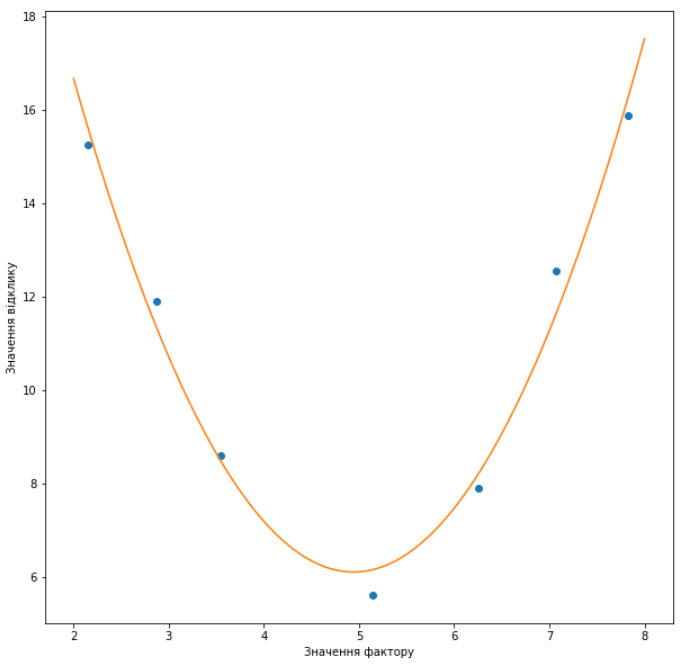
\includegraphics[scale=0.54]{plot_for_first_task_2}
\end{figure}


\subsection{На рівні значущості $\alpha = 0.05$ перевірити адекватність побудованої моделі. }

Для перевірки моделі на адекватність скористаємось F-критерієм. Він перевіряє чи є побудована модель кращою за найпростішу - константну. Висунемо основну гіпотезу: $H_0:$ константна модель та побудована не відрізняються. Тобто основна гіпотеза означає, що дисперсії похибок цих моделей однакові. Висуваємо також альтернативну гіпотезу $H_1:$ побудована модель є кращою за константну. Розглянемо статистику:

$$ \zeta = \cfrac{\frac{1}{n-1} \sum \limits_{k=1}^{n} \left(\eta_k - \bar \eta \right)^2}{\frac{1}{n-m} \|\vec{\eta} - F\vec{\beta^*}\|^2} = \cfrac{\frac{1}{n-1} \sum \limits_{k=1}^{n} \left(\eta_k - \bar \eta \right)^2}{\frac{1}{n-m} \sum \limits_{k=1}^{n}\left( \eta_k - f^*(\vec{x^{(k)}})\right)^2 } \sim F(n-1,n-m),$$

де $n$ - кількість спостережень, а $m$ - кількість невідомих параметрів. В нашому випадку $n = 7, m = 3$. 

Критична область є правосторонньою: при $\zeta_{\text{зн}} > t_{\text{кр}}$ основна гіпотеза відхиляється і модель вважається адекватною. 

Знайдемо значення статистики($\zeta_{\text{зн}}$): 

$$ (\bar \eta)_{\text{зн}}= \frac{1}{7}\left(15.24 + 11.9 +  8.6 + 5.6 + 7.9 + 12.54 + 15.88\right) \approx 11.0943$$

$$ \zeta_{\text{зн}} =  \cfrac{2}{3} \cdot \cfrac{(15.24 - 11.0943)^2  + \dots + (15.88 - 11.0943)^2}{(15.24 - 15.6168)^2 + \dots + (15.88 - 16.2824)^2}  \approx 32.2557$$

За таблицею квантилів рівня 0.95 для розподілу Фішера-Снедекора знаходимо значення $t_{\text{кр}}:$ оскільки  $n_1 = 6, n_2 = 4, \alpha = 0.05$, маємо  $t_{\text{кр}} = 6.16$. Оскільки критична область є правостороньою і $\zeta_{\text{зн}} > t_{\text{кр}}$, то на рівні значущості $\alpha = 0.05$ модель можна вважати адекватною. Оскільки модель адекватна, то її не треба замінювати на ту, яка має більший максимальний степінь. Але я вирішив побудувати ще одну, точішу, з використанням мови програмування python та бібліотек numpy і matplotlib. Вона знаходиться в додатку А(після 12 сторінки).

\subsection{Для найменшого значення параметра побудованої моделі на рівні значущості $\alpha = 0.05$ перевірити гіпотезу про його значущість.}

На рівні значущості $\alpha = 0.05$ перевіримо гіпотезу про значущість параметру $\beta_3 \Bigl( (\beta^*_3)_{\text{зн}} = 1.122124 \Bigl)$. Основною гіпотезою є $H_0: \beta_3 = 0$, альтернативною -- $H_1: \beta_3 > 0$. Критична область є правосторонньою. Розглядаємо статистику:

$$ \gamma = \cfrac{\beta^*_j}{\sqrt{(\sigma^2)^{**} \cdot a_{jj}}} \sim St_{n-m}$$

В нашому випадку $j = 3, n = 7, m = 3$, тому

$$ \gamma = \cfrac{\beta^*_3}{\sqrt{(\sigma^2)^{**} \cdot a_{33}}} \sim St_{4}$$

Знайдемо значення $\gamma_{\text{зн}}:$

$$((\sigma^2)^{**})_{\text{зн}} = \cfrac{1}{4} \left\| \vec{\eta}_{\text{зн}} - F (\vec{\beta^*})_{\text{зн}} \right\|^2  \approx 0.161934$$

$$\gamma_{\text{зн}} = \cfrac{1.122124}{\sqrt{0.161934 \cdot 0.0698}} \approx 11.4869 $$

За таблицею деяких квантилів розподілу $St_n$ знаходимо значення $t_{\text{кр}}.$ В нашому випадку $\alpha = 0.05, n = 4$, тому $t_{\text{кр}} = 2.132$ . Оскільки критична область - правостороння і $\gamma_{\text{зн}} > t_{\text{кр}}$, то ми потрапляємо в критичну область. Основна гіпотеза відхиляється, тому параметр $\beta_{3}$ є значущим.

\subsection{Побудувати прогнозований довірчий інтервал з довірчою ймовірністю $g = 0.95$ для середнього значення відклику та самого значення відклику в деякій точці, яку треба обрати самому.}

Виберемо точку $x_0 = 6.5$. Під $\vec{x}$ будемо вважати вже вибраний набір значень факторів $\vec{x} = (1, 6.5, 6.5^2)^T$

Для побудови довірчого інтервалу для середнього значення відклику використаємо статистику:

$$ \nu = \cfrac{f^*(\vec{x}) - f(\vec{x})}{\sqrt{(\sigma^2)^{**}  \vec{x}^T A^{-1} \vec{x}}} \sim St_{n-m} = St_4$$

Довірчий інтервал для середнього значення відклику має вигляд:

$$ f(\vec{x}) \in \left( f^*(\vec{x}) - t \sqrt{(\sigma^2)^{**} \vec{x}^T A^{-1} \vec{x}}, f^*(\vec{x}) + t \sqrt{(\sigma^2)^{**} \vec{x}^T A^{-1} \vec{x}} \right) $$


Обчислимо значення $\vec{x}^T A^{-1} \vec{x}$ та $f_{\text{зн}}^*(\vec{x})$:

$$ \vec{x}^T A^{-1} \vec{x} \approx \left( 1, 6.5, 6.5^2 \right) 
\begin{pmatrix}
8.2417 & -3.6636 & 0.3512 \\
-3.6636 & 1.7186 & -0.1694 \\
0.3512 & -0.1694 & 0.0171 
\end{pmatrix}
\begin{pmatrix}
1 \\
6.5 \\
6.5^2 
\end{pmatrix}
\approx 0.2755
$$

$$
f^*_{\text{зн}}(\vec{x}) \approx  35.9238 -12.071x_0 + 1.22124 x_0^2 \approx 9.0611 
$$

За таблицею значень квантилів розподілу Стьюдента знаходимо значення $t_{} = t_{0.025, 4} = 2.776$ . Отже, піставивши значення маємо:

$$ \left(9.0611  - 2.776\sqrt{0.161934 \cdot 0.2755}, 9.0611 + 2.776\sqrt{0.161934 \cdot 0.2755} \right) \approx (8.475, 9.65)$$

Отже, отримали довірчий інтервал для середнього значення відклику у точці $x_0:$ $f(\vec{x}) \in (8.475, 9.65)$ з ймовірністю 0.95.

Тепер побудуємо прогнозований інтервал з довірчою ймовірністю 0.95  для самого значення відклику. Розглянемо таку статистику:

$$ \epsilon =  \cfrac{\eta - f^{*}(\vec{x})}{\sqrt{(\sigma^2)^{**}  ( 1 + \vec{x}^T A^{-1} \vec{x}) }} \sim St_{n-m} = St_4$$

Довірчий інтервал для самого значення відклику має вигляд:

$$ \eta \in \left( f^*(\vec{x}) - t\sqrt{(\sigma^2)^{**}  ( 1 + \vec{x}^T A^{-1} \vec{x})},  f^*(\vec{x}) + t\sqrt{(\sigma^2)^{**}  ( 1 + \vec{x}^T A^{-1} \vec{x})} \right) $$

Підставимо значення:

$$ \left(9.0611  - 2.776 \sqrt{0.161934\cdot(1 +  0.2755)},  9.0611  +  2.776 \sqrt{0.161934\cdot(1 +  0.2755)} \right) \approx (7.8,  10.32) $$

Отже, отримали довірчий інтервал для значення відклику у точці $x_0:$ $\eta \in  (7.8,  10.32)$ з ймовірністю 0.95.

\subsection{Висновки}

Під час виконання першого завдання було проаналізовано вибірку. Оскільки точки на діаграмі розсіювання нагадували параболу було вибрано лінійну регресійну модель такого виду: 
$f(x) = \beta_0 + \beta_1 x + \beta_2 x^2$. Методом найменших квадратів було знайдено значення оцінок параметрів моделі. На рівні значущості $0.05$ була перевірена адекватність моделі. Було показано, що на рівні значущості $\alpha = 0.05$ модель можна вважати адекватною. Згодом був вибраний параметр найменший по модулю і була проведена перевірка його на значущість. Параметр виявся значущим. Було побудовано прогнозовані довірчі інтервали з довірчими ймовірностями рівними 0.95 для середнього значення відклику та самого значення відклику в точці $x_0 = 6.5$ ($f(\vec{x}) \in (8.475, 9.65)$ $\eta_{\text{зн}} \in  (7.8,  10.32)$). Модель на діаграмі розсіювання:


\begin{figure}[h]
\centering
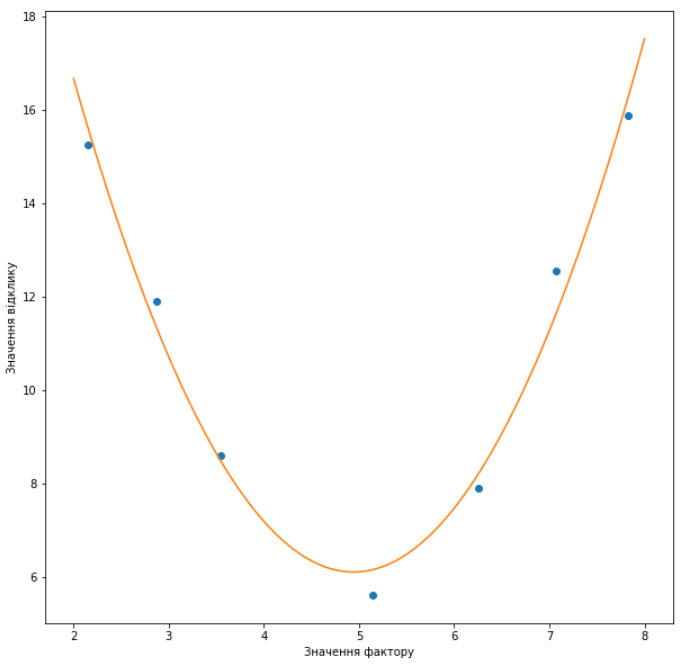
\includegraphics[scale=0.54]{plot_for_first_task_2}
\end{figure}

\newpage{}



\section{Завдання 2.}

Дана таблиця експериментальних даних.
Треба:

\begin{enumerate}
\item За методом найменших квадратів знайти оцінки параметрів двофакторної регресійної моделі.

\item На рівні значушості $\alpha = 0.05$ перевірити адекватність побудованої моделі. 

\item Для найменшого значення параметра побудованої моделі на рівні значущості $ \alpha = 0.05$ перевірити гіпотезу про його значущість. 

\item Побудувати прогнозований довірчий інтервал з довірчою ймовірністю $g = 0.95$ для середнього значення відклику та самого значення відклику в деякій точці(точку треба вибрати самому).

\item Написати висновки.
\end{enumerate}

\begin{figure}[h]
\centering
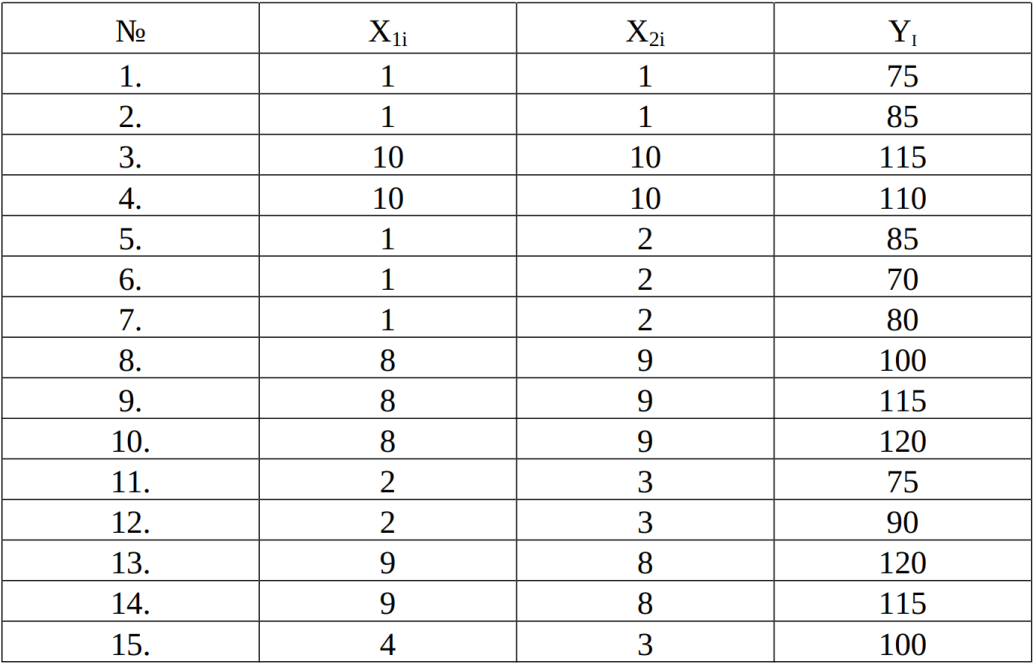
\includegraphics[scale=0.54]{table}
\end{figure}


Зобразимо тривимірну діаграму розсіювання з різних ракурсів:


\begin{figure}[h]
\centering
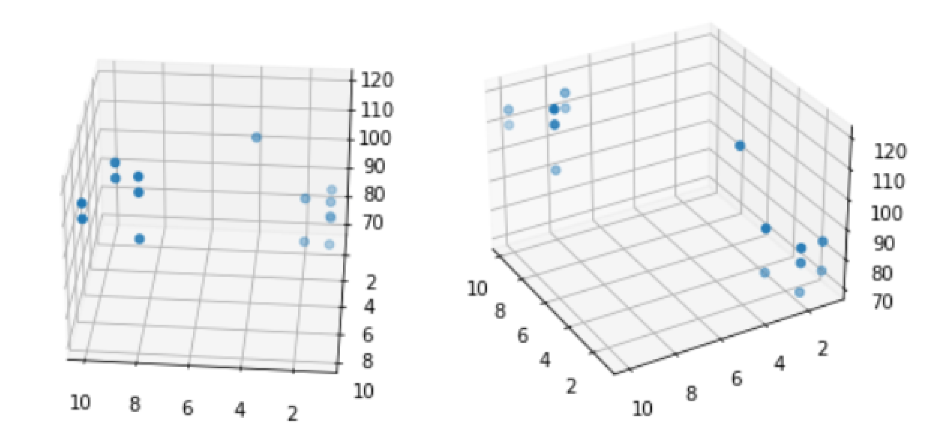
\includegraphics[scale=0.54]{plot_for_second_task_3}
\end{figure}

\newpage{}

Візуалізуємо таблицю експериментальних данних за допомогою бібліотеки мови пайтон - Pandas. Побудуємо так звану scatter\_marix. Це "матриця" елементами якої є діаграми розсіювання.  Ця матриця корисна, оскільки допомагає візуалізувати зв'язок змінними в наборі данних. 

\begin{figure}[h]
\centering
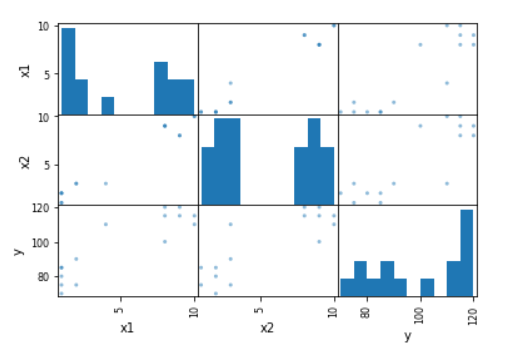
\includegraphics[scale=1]{scatter_matrix}
\end{figure}

Як бачимо, по мірі зростання $x1$ чи $x2$ зростає $y$. Видно хоч і слабку, але все таки лінійну залежність. Тому розглянемо просту лінійну двофакторну регресійну модель:

$$ f(\vec{x})= \beta_0 + \beta_1 x_1 + \beta_2 x_2 $$

\subsection{За методом найменших квадратів знайти оцінки параметрів двофакторної регресійної моделі.}

Матриця плану для вибрано моделі має вигляд:

$$
F =
\begin{pmatrix}
1 & 1 & 1 & \cdots & 1 \\
1 & 1 & 10 & \cdots & 4 \\
1 & 1 &  10 & \cdots & 3 \\
\end{pmatrix}^T
$$

Знайдемо інформаційну матрицю $A = F^T F$, а також  дисперсійну матрицю Фішера $A^{-1}$:

$$
A =  F^T F =
\begin{pmatrix}
1 & 1 & 1 \\
1 & 1 & 1 \\
1 & 10 & 10 \\
\vdots & \vdots & \vdots \\
1 & 4 & 3 
\end{pmatrix}
\cdot
\begin{pmatrix}
1 & 1 & 1 & \cdots & 1 \\
1 & 1 & 10 & \cdots & 4 \\
1 & 1 &  10 & \cdots & 3 \\
\end{pmatrix}
=
\begin{pmatrix}
15 &  75 &  80 \\
75 & 583 & 592 \\
80 & 592 & 612 \\
\end{pmatrix}
$$


$$
A^{-1} \approx
\begin{pmatrix}
0.2505 &  0.0578 & -0.0886 \\
0.0578 &   0.11  & -0.1139 \\
-0.0886 & -0.1139 &  0.1234\\  
\end{pmatrix}
$$

\newpage{}

Перевіримо деякі властивості інформаційної матриці 

\begin{enumerate}

\item Інформаційна матриця симетрична - виконується.

\item $F^T$ - матриця $3 \times 15$, $F$ - матриця $15 \times 3$, тому матриця $A = F^T F$ має мати розмірність $3 \times 3$ - виконується

\item A має бути додатньо визначеною 

$$
\begin{aligned}
&\Delta_1 = 15 > 0 \\
%
& \Delta_2 = 
\begin{vmatrix}
15 &  75  \\
75 & 583
\end{vmatrix} =3120 >0 \\
%
& \Delta_3 = 
\begin{vmatrix}
15 &  75 &  80 \\
75 & 583 & 592 \\
80 & 592 & 612 \\
\end{vmatrix}= 25280 >0 
\end{aligned}  
$$
Отже, за критерієм Сильвестра: матриця A - додатньо визначена
\end{enumerate}

Вектор значень відкликів має вигляд:

$$ \vec{\eta_{\text{зн}}} = \left(75, 85, 115, 110, \dots, 100 \right)^T$$

Як і в першому завданні, оскільки $rang F = 3$, то, щоб використовувати МНК треба зробити припущення лише про те що вектор похибок спостережень розподілений так: $\vec{\varepsilon} \sim N(\vec{0}, \sigma^2I)$. Тепер можемо знайти значення оцінок параметрів нашої моделі:

$$ \vec{\beta^*_{\text{зн}}} = A^{-1}F^T \vec{\eta_{\text{зн}}} =
 \begin{pmatrix}
0.2505 &  0.0578 & -0.0886 \\
0.0578 &   0.11  & -0.1139 \\
-0.0886 & -0.1139 &  0.1234\\  
\end{pmatrix}
\cdot 
\begin{pmatrix}
1 & 1 & 1 & \cdots & 1 \\
1 & 1 & 10 & \cdots & 4 \\
1 & 1 &  10 & \cdots & 3 \\
\end{pmatrix}
\cdot 
\left(75, 85, 115, 110, \dots, 100 \right)^T \approx
$$

$$
\approx
\begin{pmatrix}
79.0736 \\
7.7017 \\
-3.7342 
\end{pmatrix}
$$

Отримали таку модель:

$$ f_{\text{зн}}^*(\vec{x}) = 79.0736 + 7.7017x_1 -3.7342 x_2$$

Зобразимо її графік на тривимірній діаграмі розсіювання.

\begin{figure}[h]
\centering
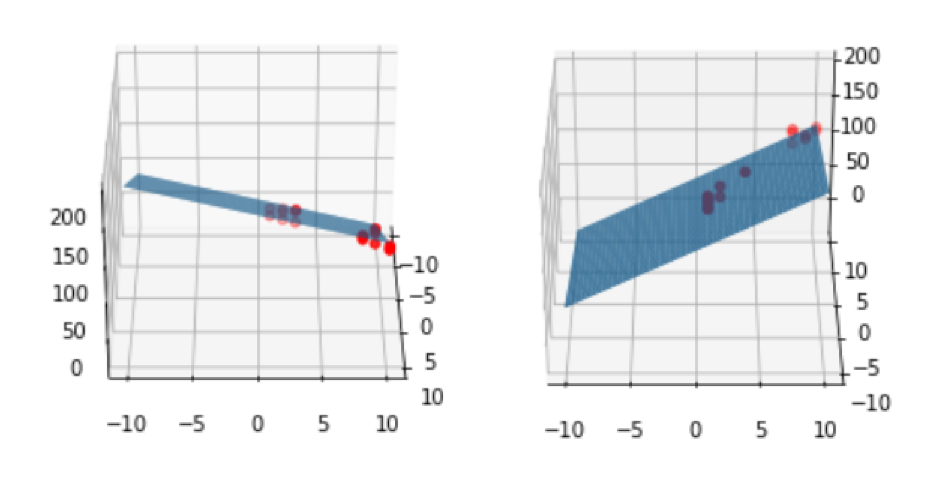
\includegraphics[scale=0.47]{plot_for_second_task_6}
\end{figure}


\subsection{На рівні значушості $\alpha = 0.05$ перевірити адекватність побудованої моделі.}

Як і в попередній задачі, будемо перевіряти адекватність моделі за F критерієм. Розглядаємо статистику:

$$ \zeta =  \cfrac{\frac{1}{n-1} \sum \limits_{k=1}^{n} \left(\eta_k - \bar \eta \right)^2}{\frac{1}{n-m} \sum \limits_{k=1}^{n}\left( \eta_k - f^*(\vec{x^{(k)}})\right)^2 } \sim F(n-1,n-m) $$

У нашому випадку $n = 15, m = 3$. Висуваємо основну гіпотезу $H_0:$ константна модель та побудована не відрізняються, а також альтернативну $H_1:$ побудована модель є кращою за константну. Знайдемо значення статистики($\zeta_{\text{зн}}$):

$$ (\bar \eta)_{\text{ зн}} = \cfrac{1}{15} \Bigl(75 + 85 + 115 + 110 + \dots + 100 \Bigl) \approx 97.667$$

$$ \zeta_{\text{зн}} = \cfrac{\frac{1}{14} \left( (75 - 97.667)^2 + \dots + (100 - 97.667)^2 \right)}{\frac{1}{12}( (75 - 83.0411)^2 + \dots + (100 - 98.678)^2 )} \approx 4.937$$

З таблиці квантилів рівня 0.95 для  розподілу Фішера-Снедекора знаходимо значення $t_{\text{кр}} = t_{14, 12} \approx 2.64$. Оскільки критична область правостороння і $\zeta_{\text{зн}} > t_{\text{кр}},$ то основна гіпотеза відхиляється і приймається альтернативна. Тобто, на рівні значущості $\alpha = 0.05$  дані не суперечать адекватності моделі. 

\subsection{Для найменшого значення параметра побудованої моделі на рівні значущості $ \alpha = 0.05$ перевірити гіпотезу про його значущість. }

На рівні значущості $ \alpha = 0.05$ перевіримо гіпотезу про значущість параметру $\beta_3 \left((\beta^*_3)_{\text{зн}} = -3.7342  \right)$.  Висуваємо основну гіпотезу $H_0:  \beta_3 = 0 $ і альтернативну $H_1: \beta_3 < 0.$. критична область - лівостороння. Розглядаємо статистику:

$$ \gamma = \cfrac{\beta^*_j}{\sqrt{(\sigma^2)^{**} \cdot a_{jj}}} \sim St_{n-m}$$

Обчислимо значення цієї статистики:

$$\gamma_{\text{зн}} = \cfrac{-3.7342 }{\sqrt{\frac{1}{12} \cdot 67.9038 \cdot 0.00004}} \approx  -1.29$$

З таблиці квантилів розподілу Стьюдента знаходимо: $t_{\text{кр}} = -t_{0.05, 12} = -1.782$. Оскільки критична область лівостороння і $t_{\text{кр}} < \gamma_{\text{зн}}$, то ми попадаємо в область прийняття гіпотези. Отже, на рівні значущості 0.05 ми приймаємо припущення, що параметр $\beta_3$ є незначущим. Таким чином маємо нову модель:

$$ \left(f_2^*(\vec{x})\right)_{\text{зн}} = 79.0736 + 7.7017x_1$$

Перевіримо її на адекватність. Знайдемо значення статистики $\zeta$. 

$$ \zeta_{\text{зн}} = \cfrac{\frac{1}{14} \left( (75 - 97.667)^2 + \dots + (100 - 97.667)^2 \right)}{\frac{1}{13}( (75 - 86.775)^2 + \dots + (100 - 109.88)^2 )} \approx 0.43$$

Тепер ми оцінюємо не 3, а 2 параметри, тому $m = 2$. Знаходимо значення: $t_{\text{кр}} = t_{14, 13} = 2.55$. Оскільки критична область правостороння, то приймається основна гіпотеза, тому модель не є адекватною на рівні значущості 0.05. Тому повертаємось до попередньої моделі:

$$ f_{\text{зн}}^*(\vec{x}) = 79.0736 + 7.7017x_1 -3.7342 x_2$$


\subsection{Побудувати прогнозований довірчий інтервал з довірчою ймовірністю $g = 0.95$ для середнього значення відклику та самого значення відклику в деякій точці(точку треба вибрати самому).}

Виберемо точку $\vec{x_0} = (2,2)^T$. $\vec{x}$ тут вважатимемо вже вибраним набором значень факторів.

\begin{enumerate}

\item Інтервал для середнього значення.

Розглядаємо статистику:

$$ \nu = \cfrac{f^*(\vec{x}) - f(\vec{x})}{\sqrt{(\sigma^2)^{**}  \vec{x}^T A^{-1} \vec{x}}} \sim St_{12}$$

Шуканий довірчий інтервал має вигляд:

$$ f(\vec{x}) \in \left( f^*(\vec{x}) - t \sqrt{(\sigma^2)^{**} \vec{x}^T A^{-1} \vec{x}}, f^*(\vec{x}) + t \sqrt{(\sigma^2)^{**} \vec{x}^T A^{-1} \vec{x}} \right) $$

Обчислимо його межі для наших даних:

$$ \vec{x^T} A^{-1}\vec{x} = 
\begin{pmatrix}
1 \\
2 \\
2 
\end{pmatrix}
\cdot
\begin{pmatrix}
0.2505 &  0.0578 & -0.0886 \\
0.0578 &   0.11  & -0.1139 \\
-0.0886 & -0.1139 &  0.1234\\  
\end{pmatrix}
\cdot \left(1, 2, 2 \right)
\approx 0.1492
$$


$$ (\sigma^2)^{**}_{\text{зн}} = \cfrac{1}{15-3} \left\|\vec{\eta}_{\text{зн}} - F \vec{\beta^*}_{\text{зн}} \right\| \approx 67.9038; \qquad
t = St_{0.025, 12} = 2.179$$

тому маємо $ f(\vec{x}) \in \left(80.073, 93.944\right) $ з ймовірністю 0.95

\item Інтервал для самого значення відклику.

Розглядаємо статистику:

$$ \epsilon =  \cfrac{\eta - f^{*}(\vec{x})}{\sqrt{(\sigma^2)^{**}  ( 1 + \vec{x}^T A^{-1} \vec{x}) }} \sim St_{n-m} = St_{12}$$

Шуканий довірчий інтервал має вигляд:

$$ \eta \in \left( f^*(\vec{x}) - t\sqrt{(\sigma^2)^{**}  ( 1 + \vec{x}^T A^{-1} \vec{x})},  f^*(\vec{x}) + t\sqrt{(\sigma^2)^{**}  ( 1 + \vec{x}^T A^{-1} \vec{x})} \right) $$

Обчислимо його межі для наших даних. Отримуємо, що $\eta \in \left(67.76, 106.2574\right)$ з  ймовірністю 0.95 
\end{enumerate}

\subsection{Висновки.}

Під час виконання другого завдання була проаналізована таблиця експериментальних даних: а саме побудована тривимірна діаграма розсіювання а також за допомогою бібліотеки pandas мови програмування python була побудована так звана scatter\_matrix. Було вирішено вибрати просту лінійну двофакторну регресійну модель: $f(\vec{x}) = \beta_0 + \beta_1 x_1 + \beta_2 x_2$. За методом найменших квадратів було знайдено значення оцінок параметрів моделі. Отримали таку модель: $ f_{\text{зн}}^*(\vec{x}) = 79.0736 + 7.7017x_1 -3.7342 x_2$ Було показано, що на рівні значущості $\alpha = 0.05$ дані не суперечать адекватності побудованої моделі. Була також проведена  перевірка найменшого по модулю параметра на значущість. Виявилося, що він є незначущим. Таким чимном ми отримали нову модель: $ \left(f_2^*(\vec{x})\right)_{\text{зн}} = 79.0736 + 7.7017x_1$. Але, оскільки вона не пройшла перевірку на адекватність, то ми повернулися до попередньої моделі. В кінці були побудовані довірчі інтервали для середнього значення відклику і самого значеняня відклику в точці $x_0 = (2, 2)$

\subsection*{Використана література:}

\begin{enumerate}
\item Електоронний конспект лекцій -- Каніовська І.Ю.
\item \href{https://neerc.ifmo.ru/wiki/index.php?title=\%D0\%9F\%D0\%B5\%D1\%80\%D0\%B5\%D0\%BE\%D0\%B1\%D1\%83\%D1\%87\%D0\%B5\%D0\%BD\%D0\%B8\%D0\%B5}{Перенавчання моделі лінійної регресії}
\end{enumerate}

\subsection*{Програмне забезпечення:}

Середовище розробки jupyter notebook. Мова програмування python, а також бібліотеки мови python: pandas, numpy, matplotlib.  
\end{document} 